\chapter{Programaci\'on lineal}

\section{Introducci\'on}

Programaci\'on lineal es el problema de minimizar o maximizar una funci\'on lineal sujeta a restricciones lineales.

Comenzamos con un ejemplo simple (\cite[Capítulo 9.3]{Cengage}. Queremos maximizar la función
$$f(x_1, x_2) = 4x_1 + 6x_2$$
sujeta a las restricciones
\begin{alignat*}{2}
   & \quad & -x_1 + x_2 &\le 11 \\
   &   \quad & x_1 + x_2 &\le 27 \\
   &   \quad & 2x_1 + 5x_2 &\le 90 \\
   & &  x_1, x_2 &\ge 0.
\end{alignat*}

Cada una de las desigualdades en las restricciones define un semiplano en $\R^2$.
Podemos graficar el conjunto de todos los puntos de $\R^2$ que cumplen todas las restricciones intersecando los semiplanos correspondientes.

\begin{center}
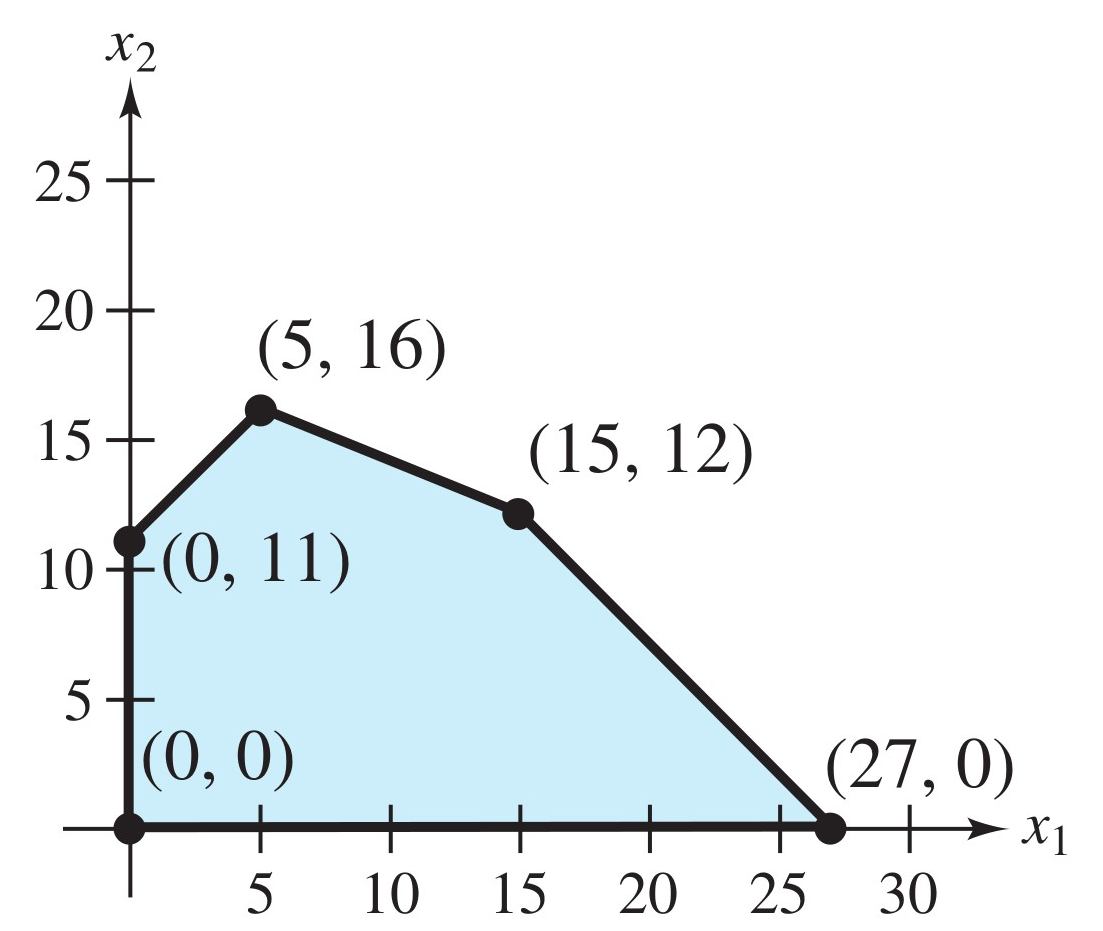
\includegraphics[scale=.2]{LP_region.png}
\end{center}

El conjunto de puntos del plano para los cuales la función toma un valor fijo $z_0$ es una recta
$$
l(z_0) = \{(x_1, x_2) : 4x_1 + 6x_2 = z_0\}.
$$

Geométricamente, si variamos el valor de $z_0$, estamos desplazando la recta obteniendo siempre rectas paralelas. En este caso particular, vemos que si desplazamos la recta hacia arriba, el valor de $z_0$ aumenta, mientras que si desplazamos la recta hacia abajo, el valor de $z_0$ disminuye.

Por lo tanto, podemos resolver el problema gráficamente, desplazando la recta hacia arriba todo lo que podamos mientras que la intersección de la recta con la figura sea no vacía.

Mediante esta resolución gráfica, podemos observar algunas propiedades del problema de programación lineal. Si la región de puntos que satisfacen las restricciones es acotada, forma un polígono, y el óptimo de la función a optimizar se alcanza en el borde del polígono. Más precisamente en un vértice del polígono (puede suceder que el óptimo se alcance también sobre todo un lado del polígono). En particular, dado que un polígono tiene una cantidad finita de vértices, el problema de programación lineal puede resolverse algorítmicamente evaluando la función objetivo sobre todos los vértices del polígono.

Estudiamos ahora el problema en mayor generalidad. Para escribir una combinación lineal de variables vamos a utilizar la notación de producto interno
$$\inner{\cb}{\xb} = c_1 x_1 + \dots + c_n x_n,$$
para $\cb, \xb \in \R^n$.
Un problema de programaci\'on lineal dado en forma est\'andar puede plantearse de la siguiente forma:
\begin{alignat*}{2}
  & \text{minimizar: } & & \inner{\cb}{\xb} \\
   & \text{sujeto a: } & \quad & \Ab\xb = \bb \\
   & & & \xb \ge 0,
\end{alignat*}
donde $\Ab \in \R^{m \times n}$, $\bb \in \R^m$, $\cb \in \R^n$ y la minimizaci\'on se realiza sobre la variable de decisi\'on $\xb \in \R^n$. La condici\'on $\xb \ge 0$ se interpreta componente a componente, es decir $x_i \ge 0$, $1 \le i \le n$. Vamos a ver que un problema donde las restricciones vienen dadas por desigualdades puede llevarse a forma estándar agregando variables auxiliares apropiadas.

\section{Conjuntos convexos y poliedros}

Comenzamos con algunas definiciones básicas.

\begin{definition}~
Dado un vector no-nulo $\ab \in \R^n$ y un escalar $b$,
  \begin{enumerate}
  \item el conjunto $\{\xb \in \R^n | \inner{\ab}{\xb} = b\}$ es un \emph{hiperplano},
  \item el conjunto $\{\xb \in \R^n | \inner{\ab}{\xb} \ge b\}$ es un \emph{semiespacio}.
  \end{enumerate}
\end{definition}

Dada una matriz $\Ab \in \R^{m \times n}$ y un vector $\bb \in \R^n$, en la condición $\Ab \xb = \bb$, cada fila $\ab_i$ de $\Ab$ impone la restricción $\inner{\ab_i}{\xb} = b_i$. El conjunto $\{\xb \in \R^n | \Ab \xb = \bb\}$ corresponde por lo tanto a una intersección de hiperplanos, que llamamos \emph{espacio afín}. Igualmente, en la condición $\Ab \xb \ge \bb$, cada fila $\ab_i$ de $\Ab$ impone la restricción $\inner{\ab_i}{\xb} \ge b_i$ y el conjunto $\{\xb \in \R^n | \Ab \xb \ge \bb\}$ corresponde a una intersección de semiespacios.

\begin{definition}
Un conjunto $S \subset \R^n$ es convexo si para todos $\xb, \yb \in S$, el segmento con vértices $\xb$ e $\yb$ está incluido en $S$. Es decir, para todo $\lambda \in [0, 1]$,
$$
\lambda \xb + (1-\lambda) \yb \in S.
$$
\end{definition}


Dado un problema de programación lineal
\begin{alignat*}{2}
  & \text{minimizar: } & & \inner{\cb}{\xb} \\
   & \text{sujeto a: } & \quad & \Ab\xb = \bb \\
   & & & \xb \ge 0,
\end{alignat*}
podemos interpretar geom\'etricamente el conjunto factible (\emph{feasible set} en ingl\'es), es decir la regi\'on sobre la que queremos minimizar $\inner{\cb}{\xb}$, como la intersecci\'on de un espacio af\'in (definido por la ecuaci\'on $\Ab\xb = \bb$) y el ortante positivo $\xb \ge 0$. Como los dos conjuntos son convexos y la intersecci\'on de conjuntos convexos es tambi\'en convexa, el conjunto factible resulta convexo.

\begin{definition}
Llamamos \emph{poliedro} a un conjunto definido por igualdades y desigualdades lineales:
$$
P = \{\xb \in \R^n \mid \Ab_1 \xb = \bb_1, \Ab_2 \xb = \bb_2\}.
$$
En el caso de que el conjunto resulte acotado, lo llamamos \emph{pol\'itopo}.
\end{definition}

Como las definiciones var\'ian seg\'un la literatura, es importante recordar entonces que para nosotros un poliedro no  necesariamente es un conjunto acotado.

\begin{ejercicio}
Dado el problema
\begin{alignat*}{2}
  & \text{minimizar: } & & 3 x_1 + 5 x_2 \\
   & \text{sujeto a: } & \quad & x_1 + x_2 = 6 \\
   & & & \xb \ge 0,
\end{alignat*}
graficar el conjunto factible, y resolver el problema.
\end{ejercicio}

\section{Variables de holgura}

Dado el problema de programación lineal
\begin{alignat*}{2}
  & \text{minimizar: } & & \inner{\cb}{\xb} \\
   & \text{sujeto a: } & \quad & \Ab\xb \le \bb \\
   & & & \xb \ge \cero,
\end{alignat*}
podemos convertir el problema a un problema con restricciones de igualdad reemplazando cada desigualdad $\inner{\ab_i}{\xb} \le b_i$ por el par de  restricciones
$$\inner{\ab_i}{\xb} + s_i =  b_i, \quad \quad s_i \ge 0,$$
donde $s_i$ es una nueva variable del problema. Estas nuevas variables se llaman \emph{variables de holgura}.

Obtenemos el problema equivalente con restricciones de igualdad
\begin{alignat*}{2}
  & \text{minimizar: } & & \inner{\cb}{\xb} \\
   & \text{sujeto a: } & \quad & \inner{\ab_1}{\xb} + s_1 = b_1 \\
   &  & \quad & \dots \\
   &  & \quad & \inner{\ab_m}{\xb} + s_m = b_m \\
   & & & \xb \ge \cero, \ssb \ge \cero,
\end{alignat*}
con $\ssb = (s_1, \dots, s_m)$.


\begin{ejercicio}
Dado el problema
\begin{alignat*}{2}
  & \text{minimizar: } & & 3 x_1 + 5 x_2 \\
   & \text{sujeto a: } & \quad & x_1 \le 1 \\
   & & & x_2 \le 1 \\
   & & & \xb \ge 0,
\end{alignat*}
\begin{enumerate}
\item graficar el conjunto factible,
\item convertirlo a un problema con igualdades agregando las variables de holgura necesarias,
\item calcular las coordenadas de los vértices del poliedro en el nuevo problema.
\end{enumerate}
\end{ejercicio}


\section{Puntos extremales, vértices y soluciones factibles básicas}

\noindent Referencia: \cite[Sección 2.2]{Bertsimas1997}.

Ya vimos geométricamente que la solución óptima de un problema de programación lineal se encuentra en una \emph{esquina} de la región factible. Veamos ahora diferentes formas de formalizar la idea de esquina.

\begin{definition}
  Dado un poliedro $P$, un vector $\xb \in P$ es un \emph{punto extremal} de $P$ si no puede escribirse como combinación convexa de dos puntos de $P$ distintos de $\xb$. Es decir, si no existen dos vectores $\yb, \zb \in P$, ambos diferentes de $\xb$, y un escalar $\lambda \in [0, 1]$ tales que $\xb = \lambda \yb + (1-\lambda) \zb$.
\end{definition}

Otra posibilidad es considerar a los puntos que son solución óptima única de un problema de programación lineal.

\begin{definition}
  Dado un poliedro $P \subset \R^n$, un vector $\xb \in P$ es un \emph{vértice} de $P$ si existe $\cb \in \R^n$ tal que
  $$\inner{\cb}{\xb} < \inner{\cb}{\yb}$$
   para todo $\yb \in P$, $\yb \neq \xb$.
\end{definition}

Es decir, $\xb$ es un vértice de $P$ si $P$ está de un lado de un hiperplano que toca a $P$ solo en $\xb$.

Una desventaja de estas definiciones geométricas es que dado un poliedro $P$ definido como intersección de hiperplanos y semiespacios, y un punto $\xb$, no es fácil verificar si se cumplen las definiciones. Veremos a continuación una definición alternativa que podemos verificar fácilmente.

Consideramos un poliedro $P$ definido por igualdades y desigualdades lineales,
$$
\begin{cases}
\inner{\ab_i}{\xb} \ge b_i, & i \in M_1 \\
\inner{\ab_i}{\xb} \le b_i, & i \in M_2 \\
\inner{\ab_i}{\xb} = b_i, & i \in M_3,
\end{cases}
$$
donde $M_1, M_2, M_3$ son conjuntos finitos de índices, $\ab_i$ son vectores en $\R^n$ y $b_i$ son escalares.

\begin{definition}
Si un vector $\xb^\star$ satisface una igualdad $\inner{\ab_i}{\xb} = b_i$ para alg\'un $i \in M_1$, $M_2$ o $M_3$, decimos que la condición correspondiente está \emph{activa} en $\xb^\star$.
\end{definition}

Si hay $n$ condiciones activas, $\xb^\star$ es solución de un sistema de $n$ ecuaciones con $n$ incógnitas. Si las $n$ ecuaciones son linealmente independientes, el sistema tiene solución única. Teniendo esto en cuenta, hacemos la siguiente definición.

\begin{definition}
Sean un poliedro $P$ definido por restricciones de igualdades y desigualdades lineales y $\xb^\star \in \R^n$.
\begin{enumerate}
\item El vector $\xb^\star$ es una \emph{solución básica} si
\begin{enumerate}
\item todas las igualdades están activas,
\item de todas las restricciones activas, hay $n$ de ellas que son linealmente independientes
\end{enumerate}
\item Si $\xb^\star$ es una solución básica que satisface todas las restricciones, decimos que $\xb^\star$ es una \emph{solución básica factible}.
\end{enumerate}
\end{definition}

Observamos que en el conjunto de restricciones podemos reemplazar una igualdad $\inner{\ab}{\xb} = b$ por dos desigualdades $\inner{\ab}{\xb} \le b$ y $\inner{\ab}{\xb} \ge b$, obteniendo un problema equivalente. Por lo tanto, la condición de ser solución básica depende de cómo está formulado el problema.

Vimos hasta ahora tres formas de capturar el mismo concepto: punto extremal, vértice y solución básica factible. Veamos ahora que las tres definiciones son equivalentes.

\begin{theorem}
Dado un poliedro $P$ no vacío y un vector $\xb^\star \in P$, las siguientes propiedades son equivalentes:
\begin{enumerate}
\item $\xb^\star$ es un punto extremal de $P$,
\item $\xb^\star$ es un vértice de $P$,
\item $\xb^\star$ es una solución básica factible de $P$.
\end{enumerate}
\end{theorem}

\begin{proof}
Por simplicidad suponemos que el poliedro está definido solo por desigualdades $\inner{\ab_i}{\xb} \ge b_i$ e igualdades $\inner{\ab_i}{\xb} = b_i$.

\textbf{Vértice $\Rightarrow$ Punto extremal.}
Para un vértice $\xb^\star \in P$ , existe $\cb \in \R^n$ tal que $\inner{\cb}{\xb^\star} < \inner{\cb}{\yb}$ para todo $\yb \in P$, $\yb \neq \xb^\star$. Si tomamos $\yb, \zb \in P$, $\yb, \zb \neq \xstar$, y $0 \le \lambda \le 1$, entonces como $\inner{\cb}{\xstar} < \inner{\cb}{\yb}$ y $\inner{\cb}{\xstar} < \inner{\cb}{\zb}$, tenemos que
$$
\inner{\cb}{\xb^\star} < \inner{\cb}{(\lambda \yb + (1-\lambda) \zb)}
$$
y por lo tanto $\xb^\star \neq \lambda \yb + (1-\lambda) \zb$.

\textbf{Punto extremal $\Rightarrow$ Solución básica factible.}
Supongamos que $\xstar \in P$ no es una solución básica factible. Vamos a ver que $\xstar$ no puede ser un punto extremal de $P$. Como $\xstar \in P$ es un punto factible, entonces $\xstar \in P$ no es solución básica. Tomamos $I = \{i \mid \inner{\ab_i}{\xstar} = b_i\}$, el conjunto de índices de las restricciones activas. Como $\xstar$ no es una solución básica, no hay $n$ vectores linealmente independientes en $\{\ab_i\}_{i \in I}$. Si construimos una matriz $\Ab$ con estos vectores como fila, esta matriz tiene rango menor que $n$ y por lo tanto existe $\db \in \R^n$ tal que $\Ab \db = \cero$, es decir, $\inner{\ab_i}{\db_i} = 0$ para todo $i \in I$.

Para $i \not\in I$, $\inner{\ab_i}{\xb} > b_i$. Tomando $\epsilon$ suficientemente pequeño, los vectores $\yb = \xstar + \epsilon \db$ y $\zb = \xstar - \epsilon \db$ también van a cumplir $\inner{\ab_i}{\yb} > b_i$, $\inner{\ab_i}{\zb} > b_i$. Y por definición de $\db$, para $i \in I$, $\inner{\ab_i}{\yb} = \inner{\ab_i}{\xstar + \epsilon \db} = b_i$ y $\inner{\ab_i}{\zb} = b_i$. Luego $\yb, \zb \in P$ y
$$\xstar = \yb + \zb,$$
por lo tanto $\xstar$ no es un punto extremal.

\textbf{Solución básica factible $\Rightarrow$ Vértice.}
Sea $\xstar$ una solución básica factible y sea $I = \{i \mid \inner{\ab_i}{\xstar} = b_i\}$. Sea $\cb = \sum_{i \in I} \ab_i$. Tenemos
$$
\inner{\cb}{\xstar} =  \sum_{i \in I} \inner{\ab_i}{\xstar} = \sum_{i \in I} b_i.
$$

Más aún, para cualquier $\xb \in P$ y cualquier $i$, se cumple $\inner{\ab_i}{\xb} \ge b_i$ y
$$
\inner{\cb}{\xb}=  \sum_{i \in I} \inner{\ab_i}{\xb} \ge \sum_{i \in I} b_i.
$$

Por lo tanto $\xstar$ es una solución óptima al problema de minimizar $\inner{\cb}{\xb}$ sobre $P$. Para concluir, observamos que la igualdad en la última fórmula se cumple si y solo si $\inner{\ab_i}{\xb} = b_i$ para todo $i \in I$. Como $\xstar$ una solución básica factible, en el conjunto $\{\ab_i\}_{i \in I}$ hay $n$ vectores linealmente independientes y por lo tanto $\xstar$ es la única solución del sistema de ecuaciones $\{\inner{\ab_i}{\xb} = b_i\}_{i \in I}$. Luego $\xstar$ es el único minimizante de $\inner{\cb}{\xb}$ en $P$ y por lo tanto es un vértice de $P$.
\end{proof}


Las dos primeras definiciones son definiciones geométricas y solo dependen del conjunto $P$ y no de las ecuaciones que lo definen. Por la equivalencia, obtenemos que la condición de solución básica factible tampoco depende de las ecuaciones que definen $P$, a diferencia de las soluciones básicas que sí pueden depender.

Obtenemos el siguiente corolario simple pero muy importante.

\begin{coro}
Dado un conjunto finito de restricciones lineales (igualdades o desigualdades), la cantidad de soluciones básicas y soluciones básicas factibles es siempre finita.
\end{coro}

\begin{proof}
Dado un sistema de $m$ igualdades y desigualdades lineales, en una solución básica $\xb^\star$ se cumplen al menos $n$ de las restricciones. A la vez, las restricciones deben ser linealmente independientes, y por lo tanto $\xb^\star$ es el único vector que satisface esas restricciones. Por lo tanto soluciones básicas distintas corresponden a distintos conjuntos de $n$ restricciones. Como la cantidad posible de conjuntos de $n$ restricciones es finita, la cantidad de soluciones básicas también.
\end{proof}

Observamos sin embargo que si bien la cantidad de soluciones básicas es siempre finita, puede ser una cantidad muy grande. Por ejemplo, el cubo
$$
\{\xb \in \R^n \mid 0 \le x_i \le 1, 1 \le i \le n\}
$$
está definido por $2n$ ecuaciones y tiene $2^n$ soluciones básicas factibles.
Esto hace que en la práctica, si bien podemos evaluar la función a optimizar en todas las soluciones básicas factibles para encontrar el óptimo, puede ser un método muy ineficiente.

\section{Poliedros en forma estándar}

\noindent Referencia: \cite[Sección 2.3]{Bertsimas1997}

Un poliedro en forma estándar está definido por las siguientes ecuaciones:
$$
P = \{\xb \in \R^n : \Ab\xb = \bb, \xb \ge 0\},
$$
donde $\Ab \in \R^{m \times n}$, es decir el poliedro está definido por $m$ igualdades y $n$ desigualdades $x_i \ge 0$.
Eliminando filas redundantes de $\Ab$, podemos suponer que las $m$ filas de $\Ab$ son linealmente independientes, y por lo tanto debe ser $m \le n$.

Recordemos que en una solución básica debe haber $n$ restricciones linealmente independientes activas, y más aún, todas las restricciones de igualdad se deben cumplir, lo que nos da $m$ restricciones. Como $m \le n$, para obtener $n$ restricciones activas, debemos elegir $n - m$ variables $x_i$ y darles valor $0$, para activar las correspondientes $n-m$ desigualdades $x_i \ge 0$.

Debemos tener cuidado que no cualquier elección de las $n-m$ variables $x_i$ nos va a dar un conjunto de $n$ restricciones linealmente independientes. En el siguiente teorema vemos las condiciones que tenemos que cumplir.

\begin{theorem}
Consideremos las restricciones $\Ab\xb = \bb$ y $\xb \ge 0$, donde suponemos que las $m$ filas de $\Ab \in \R^{m \times n}$ son linealmente independientes.
Un vector $\xb^\star \in \R^n$ es una solución básica si y solo si $\Ab\xb^\star = \bb$ y existen índices $B(1), \dots, B(m)$ tales que
\begin{enumerate}
\item las columnas $\Ab_{B(1)}, \dots, \Ab_{B(m)}$ son linealmente independientes,
\item si $i \neq B(1), \dots, B(m)$, entonces $x_i = 0$.
\end{enumerate}
\end{theorem}

Este teorema nos da un procedimiento para construir soluciones básicas de un poliedro en forma estándar.

\begin{enumerate}
\item Elegir $m$ columnas linealmente independientes $\Ab_{B(1)}, \dots, \Ab_{B(m)}$.
\item Fijar $x_i = 0$ para todo $i \neq B(1), \dots, B(m)$.
\item Resolver el sistema de $m$ ecuaciones $\Ab\xb = \bb$ para las variables $x_{B(1)}, \dots, x_{B(m)}$.
\end{enumerate}

Recordemos que en una matriz el rango fila y el rango columna coinciden, por lo tanto siempre podemos encontrar $m$ columnas independientes en $\Ab$.

Si una solución básica construida siguiendo el procedimiento cumple que todas sus coordenadas son no-negativas, entonces es una solución básica factible. Recíprocamente, podemos encontrar todas las soluciones básicas factibles de esta forma.

Si $\xb$ es una solución básica, llamamos \emph{variables básicas} a las variables $x_{B(1)}, \dots, x_{B(m)}$ y \emph{no-básicas} a las demás variables. Llamamos \emph{columnas básicas} a las columnas $\Ab_{B(1)}, \dots, \Ab_{B(m)}$. Como son linealmente independientes, forman una base de $\R^m$.

Observamos que dos conjuntos distintos de variables básicas pueden dar la misma solución básica, si algunas de las variables básicas valen también $0$. En este caso, decimos que la solución es degenerada. Para simplificar el desarrollo en este apunte, supondremos siempre que todas las soluciones básicas del problema son no-degeneradas.

\section{Existencia de puntos extremales}

En general los poliedros pueden no tener puntos extremales. Por ejemplo, un semiplano en $\R^2$ no tiene puntos extremales.
Una condición muy simple para determinar si un poliedro tiene puntos extremales es la existencia o no de líneas rectas incluidas en el poliedro.

Decimos que un poliedro $P \subset \R^n$ contiene una recta si existe un vector $\xb \in P$ y una dirección $\db \in \R^n$ tales que $\xb + \lambda \db \in P$ para todo $\lambda \in \R$.

\begin{theorem}
Dado un poliedro $P = \{\xb \in \R^n \mid \inner{\ab_i}{\xb} \ge b_i, i = 1, \dots, m\}$, las siguientes condiciones son equivalentes.

\begin{enumerate}
\item El poliedro $P$ contiene al menos un punto extremal.
\item El poliedro $P$ no contiene ninguna recta.
\item Existen $n$ vectores linealmente independientes entre los vectores $\ab_1, \ab_2, \dots, \ab_m$.
\end{enumerate}
\end{theorem}

En particular, cualquier poliedro acotado tiene puntos extremales y cualquier poliedro en forma estándar tiene puntos extremales, debido a que el ortante positivo $\{x_i \ge 0, 1 \le i \le n\}$ no contiene ninguna recta.

Ahora que ya vimos condiciones para que un poliedro tenga puntos extremales, podemos preguntarnos en qué casos un problema de programación lineal tiene soluciones óptimas y verificar que se alcanzan en los puntos extremales, como vimos intuitivamente en los ejemplos.

\begin{theorem}
Consideremos el problema de programación lineal de minimizar una funcional $\inner{\cb}{\xb}$ sobre un poliedro $P$. Si $P$ tiene al menos un punto extremal y el problema tiene solución óptima, entonces existe una solución óptima que es un punto extremal.
\end{theorem}

\begin{proof}
Completar
\end{proof}

Más aún, si el costo óptimo de la función a optimizar es finito, entonces siempre existe solución óptima.

\begin{theorem}
Consideremos el problema de programación lineal de minimizar una funcional $\inner{\cb}{\xb}$ sobre un poliedro $P$. Si $P$ tiene al menos un punto extremal entonces o bien el costo óptimo es $-\infty$ o existe un punto extremal que es óptimo.
\end{theorem}
\begin{proof}
Ver \cite[Teorema 2.8]{Bertsimas1997}
\end{proof}









\section{El método Simplex}

El método Simplex es uno de los métodos más usados en la práctica para resolver problemas de programaci\'on lineal.
A partir de las herramientas desarrolladas en las secciones anteriores, podemos derivar el método simplex en forma sencilla.

Muchos métodos de optimización se basan en un principio simple que consiste en comenzar en una solución factible cualquiera e intentar moverse a otra solución factible cercana de forma que se reduzca el costo de la función a minimizar. Si no existe ninguna solución cercana que permita mejorar la función, hemos alcanzado un mínimo local. En general, un mínimo local no tiene por qué ser un mínimo global, una función podría tener varios mínimos locales, y el mínimo global ser solo uno de ellos.

Afortunadamente, en programación lineal un mínimo local es también global, dado que estamos minimizando una función convexa sobre un conjunto convexo. El método simplex se basa en aprovechar una propiedad adicional de la programación lineal. Ya vimos que en caso de existir un mínimo, este se alcanza en un vértice del poliedro de puntos factibles. Veremos que si estamos parados en un vértice, alcanza verificar si la función objetivo decrece al movernos a alguno de los vértices vecinos (que precisaremos más adelante). Si no decrece en ninguno de los vértices vecinos, hemos encontrado un mínimo local y por lo tanto global.

Obtenemos el siguiente algoritmo
\begin{enumerate}
\item Elegir un vértice $\xb$ del poliedro $P$.
\item Para cada uno de los vértices vecinos $\{\yb_1, \dots, \yb_s\}$ de $\xb$ verificar si la función objetivo mejora en esos puntos.
\item Si no mejora en ninguno de los puntos, $\xb$ es un óptimo global y finalizamos el procedimiento.
\item Si encontramos $\yb_j$ tal que $\inner{\cb}{\yb_j} < \inner{\cb}{\xb}$, tomamos $\xb = \yb_j$ y volvemos a comenzar.
\end{enumerate}

Veremos ahora como obtener los vértices vecinos de un vértice dado, y completaremos los detalles que faltan para probar la correctitud del algoritmo.

Para todo el desarrollo del método simplex, vamos a considerar el problema en forma estándar
\begin{alignat*}{2}
  & \text{minimizar: } & & \inner{\cb}{\xb} \\
   & \text{sujeto a: } & \quad & \Ab\xb = \bb, \\
   & & & \xb \ge 0.
\end{alignat*}



\subsection{Soluciones adyacentes}

Dos soluciones básicas de un conjunto de restricciones lineales en $\R^n$ se dicen \emph{adyacentes} si existen $n-1$ restricciones linealmente independientes que están activas en ambas soluciones. Si las dos soluciones son factibles, llamamos \emph{arista} del conjunto factible al segmento que las une.

\begin{ejercicio}
Sea $P = \{\xb \in \R^n \mid \inner{\ab_i}{\xb} \ge b_i,  1 \le i \le m\}$ un poliedro y $\ub$, $\vb$ dos soluciones básicas factibles adyacentes, con $\inner{\ab_i}{\ub} = \inner{\ab_i}{\vb} = b_i$ para $1 \le i \le n-1$ y $\{\ab_1, \dots, \ab_{n-1}\}$ vectores linealmente independientes.
Probar que el segmento $L = \{\lambda \ub + (1-\lambda)\vb \mid 0 \le \lambda \le 1\}$ que une $\ub$ y $\vb$ verifica
$$
L = \{\zb \in P \mid \inner{\ab_i}{\zb} = b_i, 1\le i \le n-1\}.
$$
\end{ejercicio}

\subsection{Direcciones básicas}

En base a la definición de soluciones adyacentes, para movernos de una solución dada a una adyacente, podríamos reemplazar alguna de las variables básicas por una variable no-básica y calcular la nueva solución básica. Sin embargo, vamos a ver que al elegir cuál es la variable no-básica que vamos a convertir en básica, esto ya determina la dirección en la que debemos movernos para desplazarnos a una solución adyacente.

Sea $\xb$ una solución básica factible de un problema en forma estándar y sean $B(1), \dots, B(m)$ los índices de las variables básicas. Sea $\Bb = [ \Ab_{B(1)} \cdots \Ab_{B(m)}] \in \R^{m \times m}$ la correspondiente matriz base. En particular $x_i = 0$ para cada variable no-básica y  podemos calcular las coordenadas correspondientes a variables básicas por la fórmula
$$
\xb_B = \Bb^{-1}\bb.
$$

Para movernos a una solución adyacente en la que una variable no-básica $x_j$ pase a ser variable básica, debemos desplazarnos a un nuevo vector $$\xb + \theta \db$$
con $\theta > 0$ y $\db = (d_1, \dots, d_n)$ con $d_j =1$ y $d_i = 0$ para todos los índices $i$ distintos de $j$ de variables no-básicas. El vector $\xb_B$ de variables básicas va a cambiar a $\xb_B + \theta \db_B$ con $\db_B = (d_{B(1)}, \dots, d_{B(m)})$.

Como solo nos interesan las soluciones básicas factibles, debe cumplirse
$$
\Ab(\xb + \theta \db) = \bb,
$$
y como $\xb$ también es factible, $\Ab \xb = \bb$. Por lo tanto debe cumplirse $\Ab \db = \cero$ y esto nos permite calcular $\db_B$. En efecto,
$$
\cero = \Ab \db = \sum_{i=1}^n \Ab_i d_i = \sum_{i=1}^m \Ab_{B(i)} d_{B(i)} + \Ab_j = \Bb \db_B + \Ab_j,$$
donde $\Ab_i$ es la $i$-ésima columna de $\Ab$.

Como la matriz $\Bb$ es inversible, obtenemos
$$
\db_B = -\Bb^{-1} \Ab_j.
$$

Llamamos al vector $\db$ que acabamos de construir como la $j$-ésima dirección básica. Por construcción, las restricciones de igualdad se van a mantener mientras nos vamos en esta dirección. Para las condiciones de no-negatividad de las variables, recordemos que la variable no-básica $x_j$ aumenta y las demás variables no-básicas se mantienen en 0, por lo tanto conservan la no-negatividad. Para las variables básicas, como estamos suponiendo que todas las soluciones son no-degeneradas, las variables básicas son todas positivas y podemos tomar $\theta$ suficientemente pequeño para que se sigan cumpliendo.

Antes de calcular el valor de $\theta$ apropiado para movernos a una solución adyacente, calculamos cómo varía el costo de la función a optimizar al desplazarnos en la dirección de la $j$-ésima dirección básica.

Si $\db$ es la $j$-ésima dirección básica, la razón $\inner{\cb}{\db}$ de cambio del costo en la dirección $\db$ está dada por
$$
\inner{\cb}{\db} = \inner{\cb_B}{\db_B} + c_j,
$$
donde $\cb_B = (c_{B(1)}, \dots, c_{B(m)})$. Utilizando que $\db_B = -\Bb^{-1}\Ab_{j}$, hacemos la siguiente definición.

\begin{definition}
Sea $\xb$ una solución básica, sea $\Bb$ la matriz base asociada, y sea $\cb_B$ el vector de costos de las variables básicas. Para cada $j$, definimos el \emph{costo reducido} $\bar c_j$ de la variable $x_j$ por la fórmula
$$
\bar c_j = c_j - \inner{\cb_B}{(\Bb^{-1}\Ab_{j})}.
$$
\end{definition}

El costo reducido nos dice cuánto varía la función de costo al movernos una unidad en la dirección de la $j$-ésima dirección básica. El término $c_j$ indica el aumento del costo por unidad de la variable $x_j$ y el último término es el costo de modificar las demás variables para compensar el cambio en la variable $x_j$.

\begin{example}
\label{ex:simplex}
Consideremos el problema de programación lineal
\begin{alignat*}{2}
  & \text{minimizar: } & & \inner{\cb}{\xb} \\
   & \text{sujeto a: } & \quad & \Ab\xb = \bb \\
   & & & \xb \ge 0,
\end{alignat*}
con $\cb = (2, 0, 0, 0) \in \R^4$,
$$
\Ab = \begin{pmatrix}
1 & 1 & 1 & 1 \\
2 & 0 & 3 & 4
\end{pmatrix} \in \R^{2 \times 4}
\quad \text{ y } \quad \bb = \begin{pmatrix} 2 \\ 2 \end{pmatrix} \in \R^2.
$$

Las primeras dos columnas de $\Ab$ son $\Ab_1 = (1,2)$ y $\Ab_2 = (1, 0)$. Como son linealmente independientes podemos elegir $x_1$ y $x_2$ como variables básicas. La matriz base correspondiente es
$$
\Bb = \begin{pmatrix} 1 & 1 \\ 2 & 0 \end{pmatrix}.
$$

Tomamos $x_3 = x_4 = 0$, y calculamos los valores de $x_1$ y $x_2$: $x_1 = 1$ y $x_2 = 1$. Luego $\xb = (1, 1, 0, 0)$ es una solución básica factible no-degenerada.

Construimos una dirección básica $\db$ correspondiente a aumentar el valor de la variable $x_3$. Tenemos $d_3 = 1$ y $d_4 = 0$. Las coordenedas de $\db$ correspondientes a las variables básicas las obtenemos por la fórmula
$$
\begin{pmatrix} d_1 \\ d_2 \end{pmatrix} =
\begin{pmatrix} d_{B(1)} \\ d_{B(2)} \end{pmatrix} =
\db_B = -\Bb^{-1} \Ab_3 =
-\begin{pmatrix} 0 & 1/2 \\ 1 & -1/2 \end{pmatrix}
\begin{pmatrix} 1 \\ 3 \end{pmatrix} =
\begin{pmatrix} -3/2 \\ 1/2 \end{pmatrix}.
$$

Por lo tanto $\db = (-3/2, 1/2, 1, 0)$ y el costo de movernos en esta dirección es
$$\bar c_3 = \inner{\cb}{\db} = -\frac{3}{2} c_1 + \frac{1}{2}c_2 + c_3 = -3.$$
\end{example}


El siguiente resultado confirma la idea intuitiva que tenemos de los costos reducidos.

\begin{theorem}
Sea $\xb$ una solución básica factible asociada a una matriz base $\Bb$, y sea $\bar \cb$ el vector de costos reducidos.
\begin{enumerate}
\item Si $\bar \cb \ge 0$, entonces $\xb$ es una solución óptima.
\item Si $\xb$ es una solución óptima no-degenerada, entonces $\bar \cb \ge 0$.
\end{enumerate}
\end{theorem}

\begin{proof}\leavevmode
\begin{enumerate}
\item Suponemos $\bar \cb \ge 0$, y consideramos una solución básica factible $\yb$ arbitraria (es decir, $\yb$ es un punto arbitrario del poliedro, no necesariamente un vértice). Definimos $\db = \yb - \xb$. Como $\xb$ e $\yb$ son factibles, $\Ab \xb = \Ab \yb = \bb$ y por lo tanto $\Ab \db = \cero$.

Separando las variables básicas del resto, reescribimos la última igualdad como
$$
\Bb \db_B + \sum_{i \in N} \Ab_i d_i = \cero,
$$
donde $N$ es el conjunto de índices correspondientes a variables no-básicas. Como $\Bb$ es inversible,
$$
\db_B = -\sum_{i \in N} \Bb^{-1} \Ab_i d_i,
$$
y la variación del costo al movernos de $\xb$ a $\yb$ es
\begin{align*}
\inner{\cb}{\yb} - \inner{\cb}{\xb} = \inner{\cb}{\db} &= \inner{\cb_B}{\db_B} + \sum_{i \in N} c_i d_i \\
&= -\inner{\cb_B}{\sum_{i \in N} \Bb^{-1} \Ab_i d_i} + \sum_{i \in N} c_i d_i \\
&= \sum_{i \in N} (c_i - \inner{\cb_B}{(\Bb^{-1} \Ab_i)}) d_i = \sum_{i \in N} \bar c_i d_i.
\end{align*}


Para todo índice no-básico $i \in N$, tenemos $x_i = 0$ y como $\yb$ es factible, $y_i \ge 0$. Por lo tanto, $d_i = y_i - x_i \ge 0$ y $\bar c_i d_i \ge 0$. Concluimos que $\inner{\cb}{\yb} \ge \inner{\cb}{\xb}$ y como $\yb$ era arbitrario, $\xb$ es óptimo.

\item Si $\xb$ es una solución óptima y existe una coordenada $\bar c_j > 0$ del vector de costos reducidos, podemos desplazarnos en la dirección básica correspondiente y reducir el costo, lo que contradice la optimalidad de $\xb$.
\end{enumerate}
\end{proof}

En base a este teorema, para determinar si una solución básica factible no-degenerada es óptima, solo necesitamos chequear si todos los costos reducidos son no-negativos, lo que equivale a examinar si aumenta el costo al movernos en cada una de las $n - m$ direcciones básicas.

Por último, si encontramos una dirección básica en la cual movernos para reducir el costo, debemos calcular el mayor valor de $\theta$ que podemos tomar, lo que equivale a determinar
$$
\theta^\star = \max\{\theta \ge 0 \mid \xb + \theta \db \in P\}.
$$

Vamos a deducir una fórmula para $\theta^\star$. Como $\Ab \db = \cero$, tenemos que
$$
\Ab (\xb + \theta \db) = \Ab \xb = \bb
$$
para todo $\theta$, por lo tanto las restricciones de igual se cumplen siempre. El punto $\xb + \theta \db$ solo puede salirse del poliedro si alguna de las coordenadas se vuelve negativa. Distinguimos dos casos:

\begin{enumerate}
\item Si $\db \ge 0$ (es decir, $d_i \ge 0$ para todo $1 \le i \le n$), entonces $\xb + \theta \db \ge 0$ para todo $\theta \ge 0$. El vector $\xb + \theta \db$ nunca se vuelve no-factible, y tomamos $\theta^\star = +\infty$. El costo óptimo es $-\infty$.

\item Si $d_i < 0$ para algunos $i$, la restricción $x_i + \theta d_i > 0$ nos da la condición
$$
\theta \le -\frac{x_i}{d_i}.
$$
Estas restricciones se deben cumplir para todo $i$ tal que $d_i < 0$. Por lo tanto el mayor valor de $\theta$ que podemos tomar es
\begin{equation*}
\theta^\star = \min_{\{i \mid d_i < 0 \}}\left(-\frac{x_i}{d_i}\right).
\end{equation*}

Recordemos que para las variables $x_i$ no-básicas, o bien $d_i = 1$ si es la variable que pasa a ser variable básica, o bien $d_i = 0$, y en ambos casos $d_i \ge 0$. Por lo tanto podemos restringirnos a mirar las variables básicas en la fórmula anterior. Obtenemos
\begin{equation}
\label{eq:thetastar}
\theta^\star = \min_{\{i = 1, \dots, m \mid d_{B(i)} < 0 \}}\left(-\frac{x_{B(i)}}{d_{B(i)}}\right).
\end{equation}

Más aún, como supusimos que todas las soluciones son no-degeneradas, $x_i > 0$ para todas las variables básicas, y por lo tanto obtenemos siempre $\theta^\star > 0$.
\end{enumerate}

\begin{example}
Continuamos el Ejemplo \ref{ex:simplex}.  Obtuvimos $\xb = (1, 1, 0, 0)$, $\db = (-3/2, 1/2, 1, 0)$ y $\bar c_3 = -3$. Como $\bar c_3$ es negativo, podemos disminuir el costo de la función objetivo desplazándonos en esta dirección. Es decir, consideramos los vectores
$$
\xb + \theta \db,
$$
con $\theta > 0$. La única coordenada que decrece al desplazarnos es $x_1$, por lo que si tomamos cualquier valor de $\theta > 0$ tal que la primera coordenada se mantenga no-negativa, estaremos dentro del poliedro. El máximo valor de $\theta$ que podemos tomar es
$$
\theta^\star = -\frac{x_1}{d_1} = \frac{2}{3},
$$
y nos desplazamos a
$$
\yb = \xb + \frac{2}{3} \db = \left(0, \frac{4}{3}, \frac{2}{3}, 0\right).
$$
Las columnas correspondientes a las coordenadas no-nulas son $\Ab_2 = (1, 0)$ y $\Ab_3 = (1,3)$, y son linealmente independientes. Por lo tanto $\yb$ es una nueva solución básica factible. Como queríamos minimizar el valor de $x_1$, y tenemos la restricción $x_1 \ge 0$, hemos encontrado el costo óptimo. Para verificación, calculamos el costo reducido $\bar c_4$ por la fórmula
$$
\bar c_4 = c_4 - \inner{\cb_B}{(\Bb^{-1} \Ab_4)} = 1 - \begin{pmatrix} 1 & 0 \end{pmatrix} \begin{pmatrix} 1 & 1 \\ 0 & 3 \end{pmatrix}^{-1}
\begin{pmatrix} 1 \\ 4 \end{pmatrix} = \frac{4}{3}.
$$

Vemos que movernos en la dirección básica correspondiente va a incrementar el valor de la función objetivo y por lo tanto no debemos desplazarnos en esa dirección.
\end{example}



Una vez que determinamos $\theta^\star$, suponiendo que es finito, nos movemos a una nueva solución factible
$$
\yb = \xb + \theta^\star \db.
$$
Por la construcción que hicimos de $\db$ y $\theta^\star$, si $\ell$ es el índice que minimiza (\ref{eq:thetastar}), se cumple
$$
x_{B(\ell)} = 0 \quad \text{ y } x_j = \theta^\star.
$$

Es decir que $x_j$ reemplaza a $x_{B(\ell)}$ en el conjunto de variables básicas. Obtenemos un nuevo conjunto de índices de las variables básicas $\bar B = \{\bar B(1), \dots, \bar B(m)\}$ definidos por
$$
\bar B(i) = \begin{cases}
B(i), & i \neq \ell,\\
j, &i = \ell.
\end{cases}
$$

Llamamos $\bar \Bb$ a la nueva matriz base, formada por las columnas de $\Ab$ correspondientes a las nuevas variables básicas.

\begin{theorem}\leavevmode
\begin{enumerate}
\item Las columnas $\Ab_{B(i)}$, $i \neq \ell$, y $\Ab_j$ son linealmente independientes y, por lo tanto, $\bar B$ es una matriz base.
\item El vector $\yb = \xb + \theta^\star \db$ es una solución básica factible con matriz base asociada $\bar \Bb$.
\end{enumerate}
\end{theorem}

\begin{proof}
Ver \cite[Teorema 3.2]{Bertsimas1997}.
\end{proof}

Mediante el procedimiento descripto, pasamos de una solución básica factible a otra solución básica factible con menor costo.
Obtenemos la siguiente iteración del método simplex.

\begin{enumerate}[label = (\arabic*)]
\item Comenzamos con una solución básica factible $\xb$, correspondiente a variables básicas con índices $I = \{B(1), \dots, B(m)\}$.
\item Tomamos la submatriz $\Bb$ de $\Ab$ formada por las columnas correspondientes a las variables básicas, y calculamos los costos reducidos $$\bar c_j = c_j - \inner{\cb_B}{(\Bb^{-1} \Ab_j)}.$$
Si todos los costos son no-negativos, $\xb$ es una solución óptima y terminamos. Si no, elegimos algún $j$ tal que $\bar c_j < 0$.
\item Calculamos $\ub = -\db_B = \Bb^{-1} \Ab_j$. Si $\ub$ no tiene ninguna componente positiva, tomamos $\theta^\star = \infty$, el costo óptimo es $-\infty$ y el algoritmo termina.
\item Si alguna componente de $\ub$ es positiva, tomamos
$$
\theta^\star = \min_{\{i = 1, \dots, m \mid u_i > 0\}} \frac{x_{B(i)}}{u_i}.
$$
\item Sea $\ell$ un índice para el cuál se alcanza el mínimo. Construimos una nueva base reemplazando $B(\ell)$ por $j$. La nueva variable básica $\yb$ queda definida por
    $$
    \begin{cases}
    y_j = \theta^\star, \\
    y_{B(i)} = x_{B(i)} - \theta^\star u_i, & 1 \le i \le m, i \neq l \\
    y_i = 0 & \text{ para los índices de variables no-básicas.}
    \end{cases}
    $$
\end{enumerate}

En base a todo lo que vimos es fácil verificar que el método simplex descripto resuelve correctamente el problema de programación lineal.
En particular, esto nos permite demostrar la siguiente propiedad de los problemas de programación lineal.

\begin{theorem}
Consideremos el problema de programación lineal de minimizar una funcional $\inner{\cb}{\xb}$ sobre un poliedro $P$. Si $P$ tiene al menos un punto extremal entonces o bien el costo óptimo es $-\infty$ o existe un punto extremal que es óptimo.
\end{theorem}
%\begin{proof}
%Ver \cite[Teorema 2.8]{Bertsimas1997}
%\end{proof}









\subsection{El tableau del método Simplex}

Veremos ahora una implementación del método simplex utilizando mediante operaciones elementales de filas de una matriz, que suele llamarse \emph{tableau}.

Vamos a verlo en el siguiente ejemplo concreto:
\begin{alignat*}{2}
   & \text{maximizar: } \quad &  4 x_1 + 6 x_2 &= z\\
   & \text{sujeto a: }  \quad & -x_1 + x_2 &\le 11 \\
   &   \quad & x_1 + x_2 &\le 27 \\
   &   \quad & 2x_1 + 5x_2 &\le 90 \\
   & &  \xb &\ge 0.
\end{alignat*}

Como tenemos todas desigualdades menor o igual, agregamos variables de holgura $s_1$, $s_2$, $s_3$ y reemplazamos las desigualdades por igualdades:
\begin{alignat*}{2}
   & \text{maximizar: } \quad &  4 x_1 + 6 x_2 &= z\\
   & \text{sujeto a: }  \quad & -x_1 + x_2 +s_1&= 11 \\
   &   \quad & x_1 + x_2 +s_2&= 27 \\
   &   \quad & 2x_1 + 5x_2 +s_3&= 90 \\
   & &  \xb, \ssb &\ge 0.
\end{alignat*}

Como ya vimos, una \emph{solución básica} de un problema en forma estándar es una solución
$$(x_1, x_2, \dots, x_n, s_1, s_2, \dots, s_m)$$
 en la que \emph{a lo sumo} $m$ variables son nulas. Las variables no-nulas se llaman \emph{variables b\'asicas} de la solución. Si todas las variables son no-negativas, la solución se llama \emph{solución básica factible}.

La matriz inicial del método se construye colocando todas las ecuaciones de restricciones como filas, y una última fila con los coeficientes de la función objetivo escrita de la siguiente forma:
$$
-c_1 x_1 - c_2 x_2 - \dots - c_n x_n + 0 s_1 + \dots + 0 s_m + z = 0.
$$
En general omitimos el coeficiente de $z$ que se mantiene siempre en 1.

En el ejemplo, obtenemos el tableau
$$
\begin{array}{ccccccc}
x_1 & x_2 & s_1 & s_2 & s_3 & b & \\ \hline
-1 & 1 & 1 & 0 & 0 & 11 & s_1 \\
1 & 1 & 0 & 1 & 0 & 27 & s_2 \\
2 & 5 & 0 & 0 & 1 & 90 & s_3 \\ \hline
-4 & -6 & 0 & 0 & 0 & 0 &
\end{array}
$$

Las variables básicas al comenzar son $s_1, s_2, s_3$ y las variables $x_1$ y $x_2$ comienzan con valor $0$.

La solución básica inicial es
$$
x_1 = 0, x_2 = 0, s_1 = 11, s_2 = 27, s_3 = 90
$$
que en este caso resulta una solución básica factible.

En este momento podemos verificar si la solución que tenemos es óptima. La condición del método simplex para una solución óptima es que todos los números en la última fila sean no-negativos. En nuestro caso, tenemos dos coeficientes negativos y por lo tanto la solución no es óptima.

\subsubsection{Pivoteo}
Como la solución no es óptima, realizamos operaciones de pivoteo para obtener en sucesivos pasos mejores soluciones hasta llegar a la solución óptima.

Elegimos una nueva variable básica, que va a reemplazar a alguna de las variables básicas actuales.
Definimos
\begin{itemize}
\item Variable entrante a la variable con el menor valor (el más negativo) en la última fila, que tomamos como nueva variable básica.
\item Variable saliente a la variable con menor cociente $b_i / a_{ij}$ en la columna determinada por la variable entrante.
\item El pivot es la casilla de la matriz en la columna de la variable entrante y la fila de la variable saliente.
\end{itemize}

Finalmente, realizamos eliminación de Gauss-Jordan por filas sobre toda la matriz, tomando el pivot recién definido.

En nuestro ejemplo, la variable entrante es $x_2$ y la variable saliente es $s_1$.

Observaciones:
\begin{itemize}
\item La operación de pivoteo se corresponde con aumentar el valor de alguna de las variables que tenían valor 0. La elección de la variable entrante se hace de forma tal que un cambio en esta variable produzca un cambio mayor que el de las otras variables.
\item Para elegir la variable saliente, buscamos cuál es el máximo valor que podemos darle a la variable entrante sin violar las restricciones. En nuestro ejemplo, el mayor valor es $x_2 = 11$. Este valor nos permite encontrar soluciones factibles $(x_1, x_2)$ para las 3 restricciones. Si le diéramos un valor mayor, se violaría la primera restricción.
\end{itemize}

Al realizar el pivoteo, obtenemos el tableau
$$
\begin{array}{ccccccc}
x_1 & x_2 & s_1 & s_2 & s_3 & b & \\ \hline
-1 & 1 & 1 & 0 & 0 & 11 & x_2 \\
2 & 0 & -1 & 1 & 0 & 16 & s_2 \\
7 & 0 & -5 & 0 & 1 & 35 & s_3 \\ \hline
-10 & 0 & 6 & 0 & 0 & 66 &
\end{array}.
$$

Vemos que obtuvimos una solución mejorada
$$
(x_1, x_2, s_1, s_2, s_3) = (0, 11, 0, 16, 35)
$$
y el valor de la función objetivo es
$$
4 x_1 + 6 x_2 = 66.
$$

Esta solución no es óptima porque $x_1$ tiene signo negativo en la ultima fila, podemos aumentar el valor de $x_1$.

Tomamos $x_1$ como variable saliente y calculando los cocientes, tomamos $s_3$ como variable saliente.

Al aplicar Gauss-Jordan obtenemos
$$
\begin{array}{ccccccc}
x_1 & x_2 & s_1 & s_2 & s_3 & b & \\ \hline
0 & 1 & 2/7 & 0 & 1/7 & 16 & x_2 \\
0 & 0 & 3/7 & 1 & -2/7 & 6 & s_2 \\
1 & 0 & -5/7 & 0 & 1/7 & 5 & s_3 \\ \hline
0 & 0 & -8/7 & 0 & 10/7 & 116 &
\end{array}.
$$

Esta solución no es óptima porque $s_3$ tiene signo negativo en la ultima fila, podemos aumentar el valor de $s_3$.
Tomando $s_3$ como variable entrante y $s_2$ como variable saliente, obtenemos luego de pivotear:
$$
\begin{array}{ccccccc}
x_1 & x_2 & s_1 & s_2 & s_3 & b & \\ \hline
0 & 1 & 0 & -2/3 & 1/3 & 12 & x_2 \\
0 & 0 & 1 & 7/3 & -2/3 & 14 & s_2 \\
1 & 0 & 0 & 5/3 & -1/3 & 15 & x_1 \\ \hline
0 & 0 & 0 & 8/3 & 2/3 & 132 &
\end{array}.
$$


Encontramos la solución óptima del problema
$$
(x_1, x_2, s_1, s_2, s_3) = (15, 12, 0, 14, 0)
$$
con valor de la función objetivo
$$
4 x_1 + 6 x_2 = 132.
$$







\section{El problema dual}

\noindent Referencia principal: \cite[Capítulo 4]{Bertsimas1997}.

Una de las propiedades m\'as interesantes de la programaci\'on lineal es que a cada problema primal en forma estándar
\begin{alignat*}{2}
  & \text{maximizar: } & & \inner{\cb}{\xb}  \\
   & \text{sujeto a: } & \quad & \Ab \xb = \bb, \\
   &&& \xb \ge 0
\end{alignat*}
podemos asociarle un problema dual de la siguiente forma:
\begin{alignat*}{2}
  & \text{maximizar: } & & \inner{\yb}{\bb}  \\
   & \text{sujeto a: } & \quad & \Ab^T \yb \le \cb, \\
\end{alignat*}
que guarda relaciones muy fuertes con el problema primal.

\subsection{Motivación}

Consideremos el problema en forma estándar
\begin{alignat*}{2}
  & \text{minimizar: } & & \inner{\cb}{\xb}  \\
   & \text{sujeto a: } & \quad & \Ab \xb = \bb \\
   & & & \xb \ge 0,
\end{alignat*}
que llamamos \emph{problema primal}, y notamos $\xb^\star$ a una solución óptima que suponemos que existe.

Podemos relajar este problema reemplazando la restricción $\Ab\xb = \bb$ por una penalidad $\inner{\yb}{(\bb - \Ab\xb)}$, donde $\yb$ es un vector de precios del mismo tamaño que $\bb$. Obtenemos entonces el siguiente problema:
\begin{alignat*}{2}
  & \text{minimizar: } & & \inner{\cb}{\xb} + \inner{\yb}{(\bb - \Ab\xb)}, \\
   & \text{sujeto a: } & \quad & \xb \ge \cero.
\end{alignat*}

Llamamos $g(\yb)$ al costo óptimo en función de $\yb$ del problema relajado. Como tenemos más libertad en la elección de variables en el problema relajado, esperamos que $g(\yb)$ sea menor o igual que el costo óptimo $\inner{\cb}{\xb^\star}$ del problema primal. En efecto,
$$
g(\yb) = \min_{\xb \ge 0} \left\{ \inner{\cb}{\xb} + \inner{\yb}{(\bb-\Ab\xb)}\right\} \le \inner{\cb}{\xb^\star} + \inner{\yb}{(\bb - \Ab\xb^\star)} = \inner{\cb}{\xb^\star},
$$
donde usamos para la última desigualdad que $\xb^\star$ es una solución óptima del problema primal y por lo tanto $\Ab\xb^\star = \bb$.

Por lo tanto, para cualquier vector $\yb$, $g(\yb) \le \inner{\cb}{\xb^\star}$ y el valor de $g(\yb)$ es una cota inferior del costo óptimo $\inner{\cb}{\xb^\star}$ del problema primal. Queremos hallar la mejor cota posible, es decir, queremos hallar el vector $\yb$ que maximice $g(\yb)$. Este problema se conoce como el \emph{problema dual}, que podemos plantear en la forma:
\begin{alignat*}{2}
  & \text{maximizar: } & & g(\yb), \\
   & \text{sujeto a: } & \quad & \text{ninguna restricción}.
\end{alignat*}

El resultado principal de la teoría de dualidad afirma que el costo óptimo del problema dual es igual al costo óptimo $\inner{\cb}{\xb^\star}$ del problema primal. En otras palabras, si elegimos el valor de $\yb$ para el cual $g(\yb)$ es máximo, la posibilidad de violar las restricciones $ \Ab\xb = \bb$ no es de ninguna ayuda.

Por la definición de $g(\yb)$,
$$
\begin{aligned}
g(\yb) = \min_{\xb \ge 0} \left\{ \inner{\cb}{\xb} + \inner{\yb}{(\bb-\Ab\xb)}\right\}
&= \inner{\yb}{\bb} + \min_{\xb \ge 0} \left\{ \inner{\cb}{\xb} - \inner{\yb}{(\Ab\xb)} \right\} \\
&= \inner{\yb}{\bb} + \min_{\xb \ge 0} \left\{ \inner{\cb}{\xb} - \inner{(\Ab^T\yb)}{\xb} \right\} \\
&= \inner{\yb}{\bb} + \min_{\xb \ge 0} \left\{ \inner{(\cb - \Ab^T\yb)}{\xb} \right\},
\end{aligned}
$$
recordando que $\inner{\xb}{(\Ab\yb)} = \xb^T \Ab \yb = (\Ab^T \xb)^T \yb = \inner{(\Ab^T \xb)}{\yb}$.

Ahora bien, notemos que
$$\min_{\xb \ge 0} \left\{ \inner{(\cb - \Ab^T\yb)}{\xb} \right\} = \begin{cases}
0 & \text{si } \cb - \Ab^T\yb \ge \cero, \\
-\infty, & \text{en otro caso.}\end{cases}
$$

Como queremos maximizar $g(\yb)$, podemos quedarnos solo con los casos para los que $g(\yb) \neq -\infty$. Concluimos que el problema dual es equivalente al problema
\begin{alignat*}{2}
  & \text{maximizar: }  & \quad & \inner{\yb}{\bb},   \\
   & \text{sujeto a: }  &       & \Ab^T\yb \le \cb. \\
\end{alignat*}

En resumen, definimos un vector $\yb$ de parámetros o variables duales, y para cada elección de $\yb$ podemos encontrar una cota inferior para costo óptimo del problema primal. El problema dual consiste en maximizar esa cota, es decir, obtener la cota mas precisa posible. Para algunos vectores $\yb$, la cota que obtenemos es $-\infty$, que no tiene utilidad. Por lo tanto, nos restringimos a las elecciones de $\yb$ que nos dan cotas no triviales, y eso nos da las restricciones del problema dual.

\subsection{Teoremas de dualidad débil y fuerte}

A partir del razonamiento anterior, deducimos el siguiente resultado

\begin{theorem}[Dualidad débil]
Si $\xb$ es una solución factible del problema primal y $\yb$ es una solución factible del problema dual, entonces
$$
\inner{\yb}{\bb} \le \inner{\cb}{\xb}.
$$
\end{theorem}

Si bien este resultado es muy simple, tiene consecuencias interesantes.

\begin{coro}~
\begin{itemize}
\item Si el costo óptimo del problema primal es $-\infty$, entonces el problema dual no es factible.
\item Si el costo óptimo del problema dual es $+\infty$, entonces el problema primal no es factible.
\end{itemize}
\end{coro}


\begin{coro}
Sean $\xb^\star \in \R^n$ e $\yb^\star \in \R^m$ soluciones factibles de los problemas primal y dual respectivamente, y supongamos que $\inner{\yb^\star}{\bb} = \inner{\cb}{\xb^\star}$. Entonces $\xb^\star$ y $\yb^\star$ son soluciones óptimas de los problemas primal y dual respectivamente.
\end{coro}

Enunciamos ahora el resultado principal de la teoría dual de programación lineal.

\begin{theorem}[Dualidad fuerte]
Si un problema primal de programación lineal tiene solución óptima, entonces también el problema dual tiene solución óptima, y los respectivos costos óptimos son iguales.
\end{theorem}

\begin{proof}
  Si aplicamos el método Simplex al problema primal
\begin{alignat*}{2}
  & \text{minimizar: } & \quad & \inner{\cb}{\xb}  \\
  & \text{sujeto a: }   & & \Ab \xb = \bb \\
  & & & \xb \ge 0,
\end{alignat*}
vamos a obtener una solución óptima $\xb$ con base $\Bb$. Tomamos $\xb_B = \Bb^{-1}\bb$ el vector de los valores óptimos de las variables básicas.
El vector de costos reducidos es
$$\cb^T - \cb_B^T \Bb^{-1} \Ab,$$
donde $\cb_B^T$ es el vector de costos (coeficientes) de las variables básicas.
Como $\xb$ es una solución óptima,
$$\cb^T - \cb_B^T \Bb^{-1} \Ab \ge 0.$$

%($\pb^T = \cb_B^T \Bb^{-1}$)
Definimos ahora $\yb \in \R^m$ tal que $\yb^T = \cb_B^T \Bb^{-1}$. Vemos que $\yb^T \Ab  \le \cb^T$, o equivalentemente $\Ab^T \yb \le \cb$, y por lo tanto $\yb$ es una solución factible del problema dual
\begin{alignat*}{2}
  & \text{maximizar: } & \quad  & \inner{\yb}{\bb} \\
  & \text{sujeto a: }  & & \Ab^T \yb \le \cb.
\end{alignat*}

Más aún,
$$
\inner{\yb}{\bb} = \inner{(\Bb^{-1})^T \cb_B}{\bb} = \inner{\cb_B}{\Bb^{-1} \bb} = \inner{\cb_B}{\xb_B} = \inner{\cb}{\xb}.
$$
Por lo tanto, por dualidad débil, $\yb$ es una solución optima del problema dual y el costo óptimo dual coincide con el costo óptimo primal.
\end{proof}



%Veamos un ejemplo.
%
%\begin{example}
%Consideramos el problema
%\begin{align*}
%   \text{minimizar: } &  x_1 - 8 x_2 \\
%    \text{sujeto a: } & \left\{
%   \begin{array}{rcl}
%   -x_1 + 3x_2 + x_3 & = & 4, \\
%   4x_1 -  x_2 + x_4 & = & 6, \\
%   \xb & \ge &  0.
%   \end{array}
% \right.
%\end{align*}
%
%El conjunto factible es un poliedro de 2 dimensiones en $\R^4$. Como estamos minimizando una funci\'on que depende solo de las dos primeras variables, podemos proyectar este conjunto en el plano $(x_1, x_2)$. Obtenemos el pol\'igono de la Figura 2.1.
%
%Para resolver el problema, graficamos la recta $x_1-8x_2 = 0$. Sobre todos los puntos en esa recta, la funci\'on objetivo toma el valor $0$. Anal\'ogamente, si trazamos una recta paralela, la funci\'on objetivo tomar\'a un valor constante en esa recta. Si la recta se desplaza hacia la derecha el valor de la funci\'on aumentar\'a y si la desplazamos hacia la izquierda el valor disminuir\'a.
%Por lo tanto, debemos desplazarla hacia la izquierda todo lo que sea posible sin que haya interesecci\'on vac\'ia entre la recta y el pol\'igono.  Concluimos que el m\'inimo se alcanza en el punto $(x_1, x_2) = (2,2)$ y resolviendo los valores de $x_3$ y $x_4$ obtenemos que el m\'inimos es $\xb^\star = (2,2,0,0)$.
%
%
%\end{example} 